

\documentclass[12pt,a4paper]{article}
\newcommand\persiangloss[2]{#1\dotfill\lr{#2}\\}
\usepackage{graphicx}
\usepackage{xcolor}
\usepackage{listings}
\usepackage{indentfirst}
\usepackage{float}
\usepackage[pagebackref=false,colorlinks,linkcolor=blue,citecolor=magenta]{hyperref}
\usepackage{xepersian}
\settextfont{XB Niloofar}
\definecolor{vgreen}{RGB}{104,180,104}
\definecolor{vblue}{RGB}{49,49,255}
\definecolor{vorange}{RGB}{255,143,102}

\lstdefinestyle{verilog-style}
{
	language=Verilog,
	basicstyle=\small\ttfamily,
	keywordstyle=\color{vblue},
	identifierstyle=\color{black},
	commentstyle=\color{vgreen},
	numbers=left,
	numberstyle=\tiny\color{black},
	numbersep=10pt,
	tabsize=8,
	moredelim=*[s][\colorIndex]{[}{]},
	literate=*{:}{:}1
} 



\begin{document}
	\thispagestyle{empty}
	\vspace*{0mm}
	\centerline{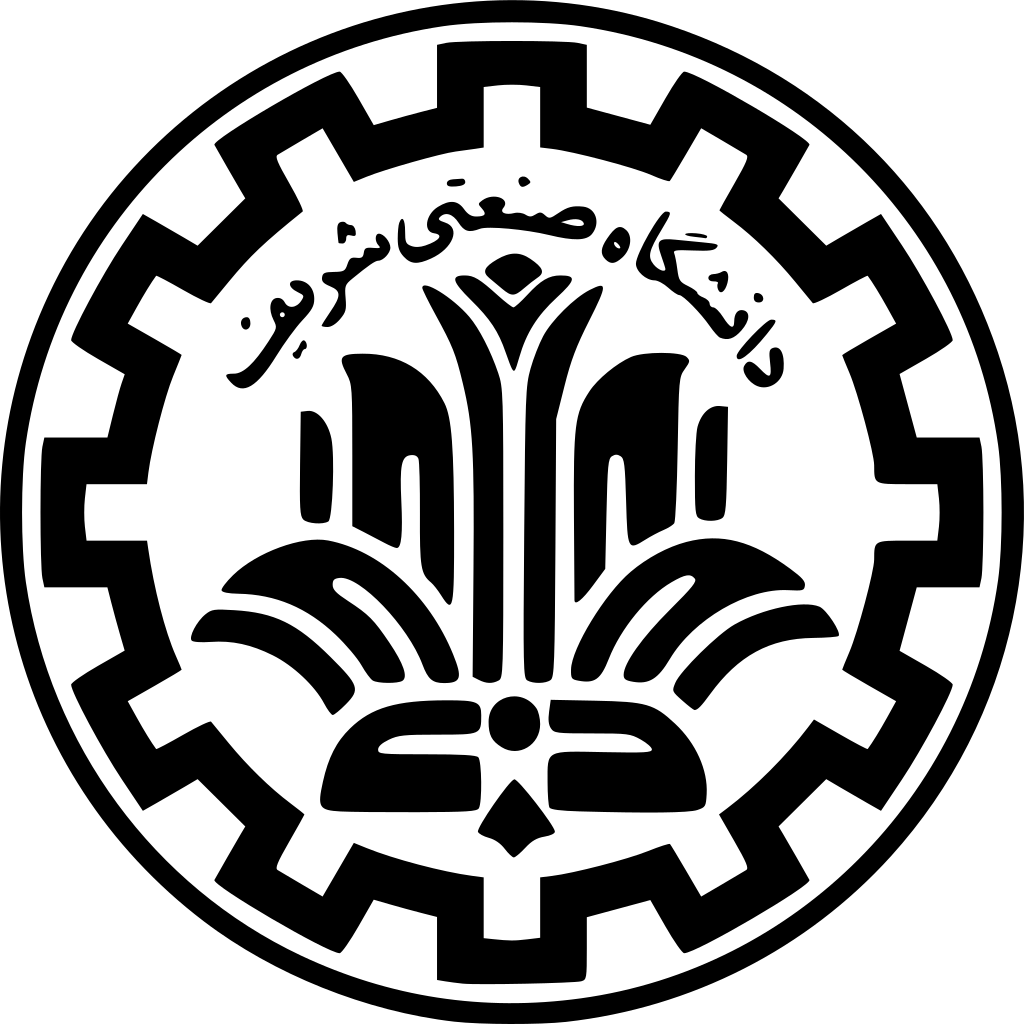
\includegraphics[height=4cm]{logo.png}}
	\vspace*{5mm}
	\begin{center}
		{\Huge
لوستر هوشمند - گزارش سوم
}
\\[1cm]
آزمایشگاه سخت‌افزار
\\[1cm]
دانشکده مهندسی کامپیوتر
\\[4cm]
{\large
محمدرضا عبدی ۹۷۱۱۰۲۸۵

حمیدرضا کامکاری ۹۷۱۱۰۱۷۷

یگانه قره‌داغی 97106216
}
	\\[5cm]
	اردیبهشت ۱۴۰۱
	\end{center}
\newpage

\section*{گزارش سوم}
هدف از این آزمایش این هفته، بستن یک لوستر شامل ۴۰ قطعه \lr{LED}، اتصال آن به منبع خارجی و همچنین کنترل آن با ترانزیستور است.

در مرحله اول، مدار آردویینو شامل سنسور هفته گذشته را بر اساس شماتیک زیر تکمیل می‌کنیم. از ترانزیستور \lr{MOSFET IRF640} برای کنترل و یک باتری ۵-۶ ولتی به عنوان منبع خارجی استفاده می‌کنیم.

 \begin{figure}[H]
 	\centering
 	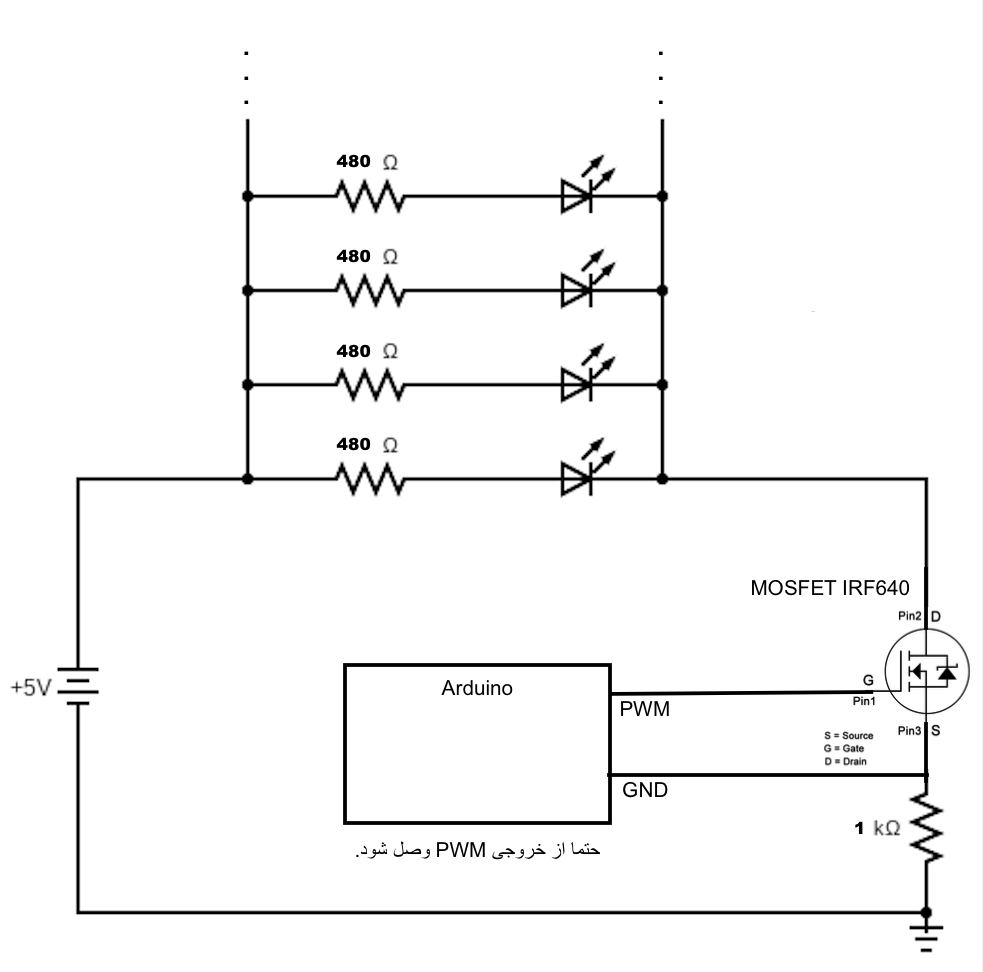
\includegraphics[scale=0.7]{figs/schematics.png}
 	\caption{
 		شماتیک مدار
 	}
 	\label{fig:schema}
 \end{figure}
 
در این مدار، \lr{LED} ها به باتری وصل هستند و خروجی \lr{PWM} به گیت کنترل ترانزیستور \lr{MOSFET IRF640} متصل است. می‌دانیم که \lr{PWM} به کمک روشن و خاموش کردن سریع می‌تواند روشنایی را کنترل کند. در اینجا، بجای اتصال مستقیم \lr{PWM} به \lr{LED} ها، به گیت ترانزیستور متصل شده و آن را به سرعت قطع و وصل می‌کند. یعنی ترانزیستوری میان باتری و \lr{LED} است که سرعت قطع و وصل کردن آن با \lr{PWM} تنظیم می‌شود.

در شکل‌های زیر می‌توان مدار بسته شده و نتیجه تغییر روشنایی \lr{LED} ها بخاطر تغییر روشنایی دریافتی سنسور را مشاهده کرد.

 \begin{figure}[H]
	\centering
	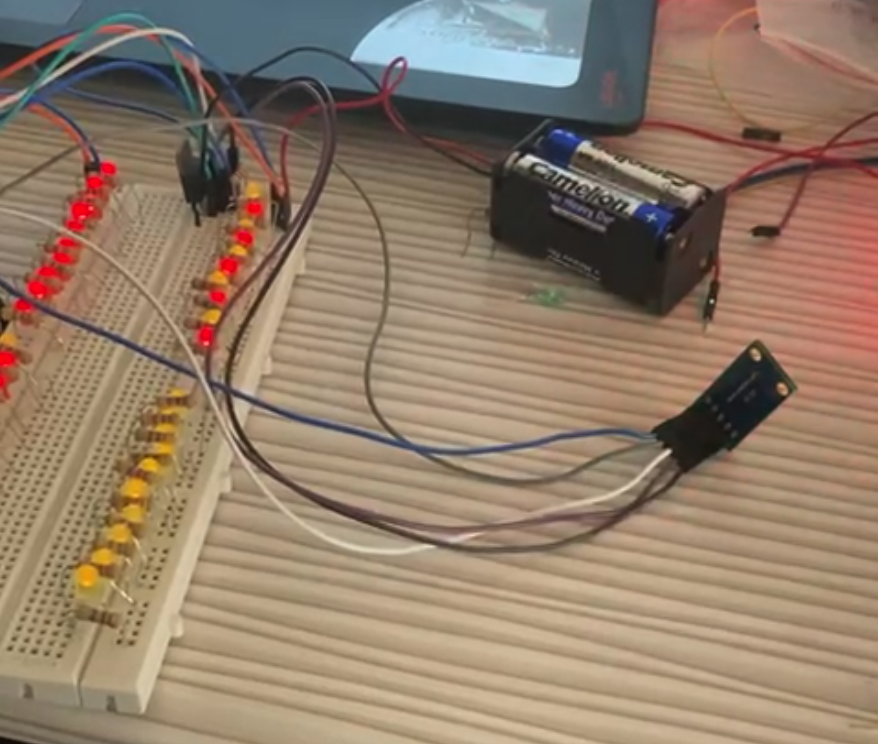
\includegraphics[scale=0.57]{figs/on.png}
	\caption{
		مدار لوستر قبل از انداختن نور بر روی سنسور روشنایی
	}
	\label{fig:schema1}
\end{figure}

 \begin{figure}[H]
	\centering
	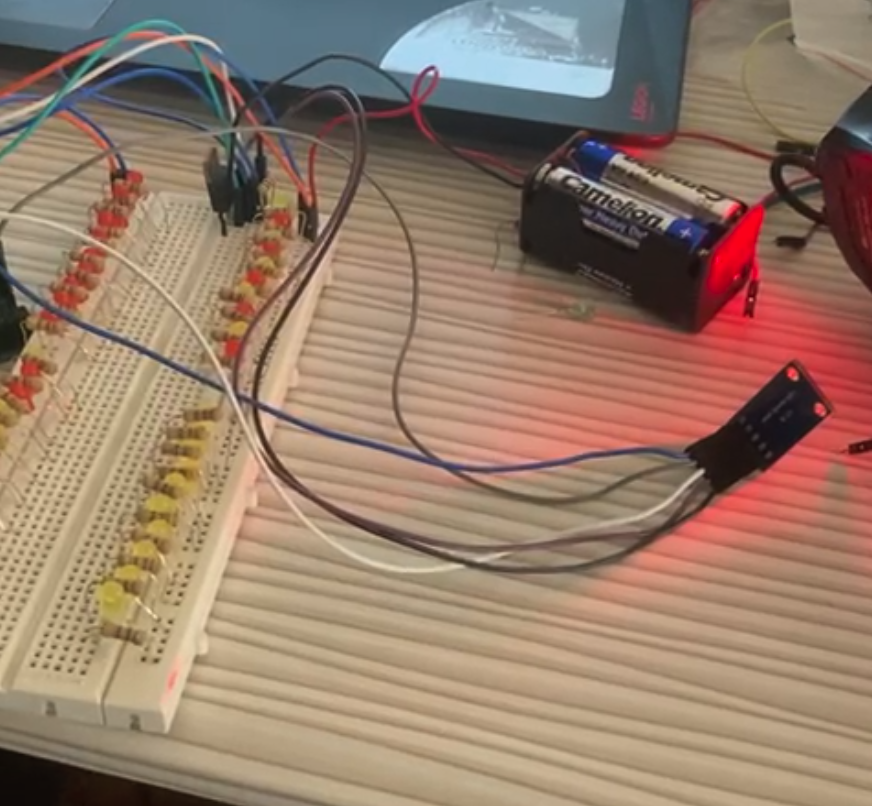
\includegraphics[scale=0.57]{figs/off.png}
	\caption{
		مدار لوستر بعد از انداختن نور بر روی سنسور روشنایی. مشاهده می‌کنیم که نور \lr{LED} ها کاهش می‌یابد.
	}
	\label{fig:schema2}
\end{figure}

در ادامه نیز می‌توان کد استفاده شده برای این قسمت را مشاهده کرد. تغییرات اندک در کد برای تنظیم دقیق‌تر و هماهنگ‌تر کردن بازه تغییرات روشنایی با نور اتاق است. اکثر تغییرات اعمال شده در گزارش این هفته به صورت پیاده‌سازی سخت‌افزاری بوده‌ است.
\begin{latin}
	\lstinputlisting[style={verilog-style}]{src/sensor-LED.ino}
\end{latin}

\end{document}